\chapter{Some Chapter Name to be changed}

\section{Diffusion Models}
\subsection{Forward Diffusion Process}

\begin{figure}[h]
    \centering
    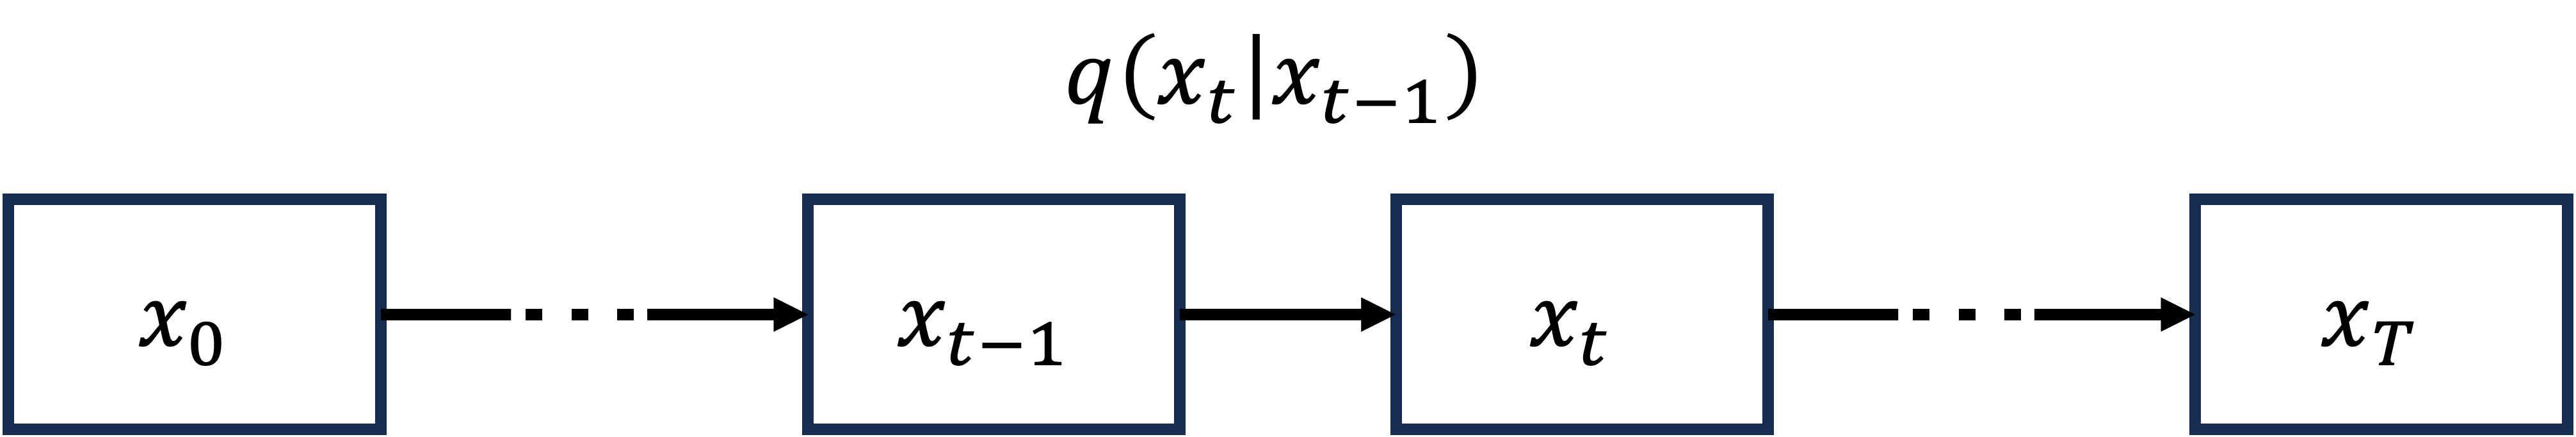
\includegraphics[width=\textwidth]{img/forward_diffusion.png}
    \caption{Forward Diffusion Process: An image is iteratively destroyed by adding normally distributed noise, 
    according to a schedule. This represents a Markov process where the transition probability $q(x_t|x_{t-1})$ 
    is equal to $\mathcal{N}$}
    \label{fig:forward_diffusion}
\end{figure}

\begin{figure}
    \centering
    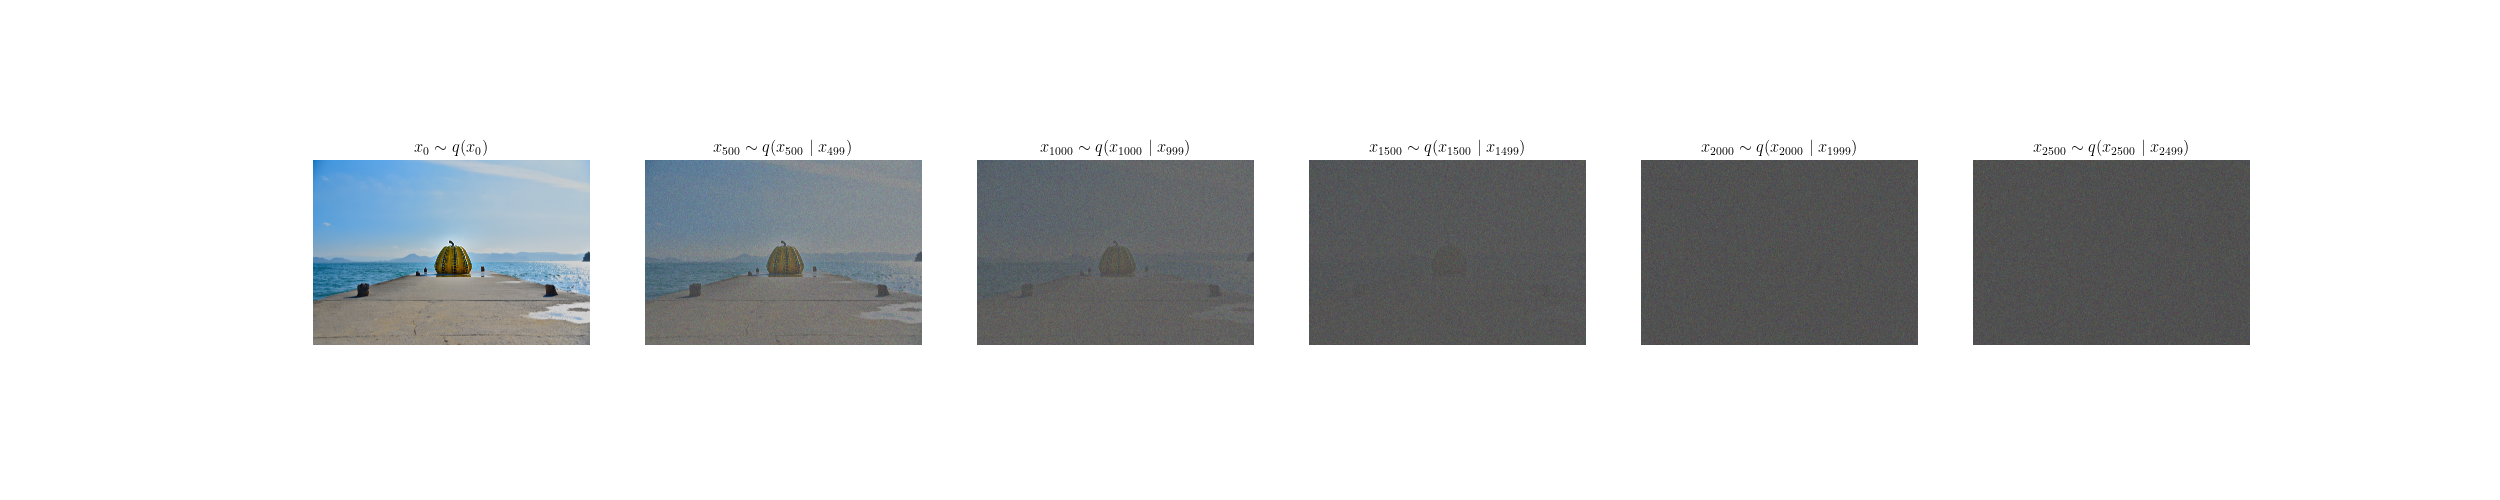
\includegraphics[width=\textwidth]{img/forward_naoshima.png}
    \caption{Example of image destruction: Forward Diffusion Process iteratively destroys according to a linear $\beta$ schedule.
    The indices give the time step in the iterative destruction process.}
\end{figure}